\newpage
\section{Information, Entropy, and Computational Complexity}

\subsection{Information is a Physical Entity}

\subsubsection{Quantifying Information}
If $X$ is a random variable over a set of events $x$ such that event $x$ occurs with probability $p_x$ , then the \hl{Shannon entropy} of event $x$ is --- $\log_2(p_x )$.


\subsubsection{A Thermodynamics Problem}
That is to say, if there are $M$ different positions to locate a molecule in the final state, there are only $p_1 M$ positions for it in the initial state.

\subsubsection{Information is Physical}
If we consider a set of possible events whose probabilities of occurrence are $p_1, p_2, \dots , p_n$, the average information is
\begin{align*}
    H=\langle I(p_i) \rangle \sim -\sum_{i=0}^n p_i\log_2 p_i
\end{align*}


Erasure is irreversible! To erase, we must dissipate heat in
the surroundings. The entropy of the surroundings must go
up by at least $k_B \ln 2$. This result, which demonstrates the intimate link between thermodynamics and information
theory, has been verified experimentally. (信息的擦除会产生热量, 这是信息与热力学的联系)

\subsubsection{Data Compression}
In general, we model a set of data to be compressed by a
random variable X . The Shannon entropy of X is then
defined as the expected logarithm of the probability:
\begin{align*}
    H(X)=-\sum_x P(X=x)\log_2 P(X=x)
\end{align*}
The probability of finding a sequence $X_1, X_2, \dots , X_n$ is
\begin{align*}
    P(X_1, X_2, \dots , X_n)=\prod_i P(X_i) \approx \prod_x P(X=x)^{nP(X=x)}
\end{align*}

The information content is approximately
% \begin{align*}
%     -\log_2 P(X_1, X_2, \dots , X_n)=&-n\sum_x P(X=x)\log_2 P(X=x)\\
%     =&H(X)
% \end{align*}
% Hence,
\begin{align*}
    P(X_1, X_2, \dots , X_n)=2^{-nH(x)}
\end{align*}
This shows that there are at most $2^{nH}$ typical sequences,
and, hence, it only requires $nH(X )$ bits to encode them.

\subsection{Computational Complexity}
\begin{figure}[H]
    \centering
    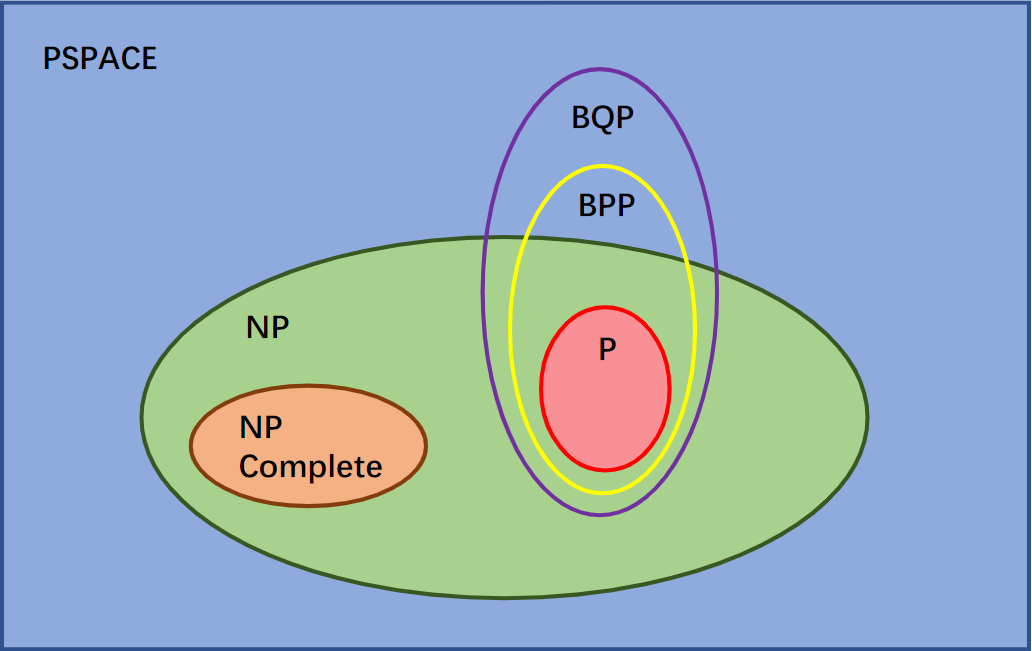
\includegraphics[width=0.309\textwidth]{QI1/Problems}
    \caption{Problems}
\end{figure}

\begin{enumerate}
    \item Information and Physics
    \item Computational Complexity
\end{enumerate}

\subsubsection{Decision Problems: P vs NP}
Most computational problems can be formulated as decision problems, whose answer is yes or no. 

\begin{itemize}
    \item P class: Problems can be solved by Polynomial time algorithm. 
    \item NP class: Problems for which a solution can be checked in Polynomial time. 
    \item NP-Complete Problem: If any of these probelms can be solved by polynomial worst-case time algorithm, then all can be solvev by polynomial worst-case time algorithms.
\end{itemize}


\subsubsection{Randomness}
A problem is in BPP (bounded-error probabilistic polynomial time) if there is an algorithm for it that has the following properties: 
\begin{itemize}
    \item It is allowed to flip coins and make random decisions.
    \item It is guaranteed to run in polynomial time.
    \item On any given run of the algorithm, it has a probability of at most 1/3 of giving the wrong answer, whether the answer is YES or NO. 
\end{itemize}

Strong Church-Turing Thesis: Any model of computation can be simulated on a probabilistic Turing machine with at most a polynomial increase in the number of elementary operations required.

\quad

\subsubsection{Quantum Randomness}
A quantum information processor differs from a classical
one (a Turing machine) in two important ways: 
\begin{enumerate}
    \item The input can be prepared not only in the binary form, but also in any superposition state.
    \item Intervention (such as examine the state of the machine) could modify the state of the quantum machine, and it would not be possible to resume the processing operation. 
\end{enumerate}

In many ways, quantum mechanics generalizes real probability to complex probability amplitudes. One can generalize the classical BPP class to BQP. 

\href{https://quantumalgorithmzoo.org}{quantumalgorithmzoo} (or, \href{https://www.qtumist.com/quantum-algorithm-zoo}{quantum-algorithm-zoo} in Chinese).

\subsection{Quantum Computing Milestones}
\begin{itemize}
    \item [1994] Peter Shor’s algorithm for factoring integers ignited a tremendous increase of interest in quantum computing.
    \item [2018] Google declared quantum supremacy, the potential ability of quantum computing devices to solve problems that classical computers practically cannot.
    \item [2019] IBM launched first 20-qubit commercial quantum computer named Q System One. Organizations started to prepare for the second quantum revolution by education in quantum engineering.
\end{itemize}